\documentclass[10pt,spanish,aspectratio=1610]{beamer}
\usepackage[utf8]{inputenc}
\usepackage{amsmath}
\usepackage{graphicx}
\usepackage{amssymb}
\usepackage[spanish]{babel}
\spanishdecimal{.}
\usepackage{subfig}
\usepackage{fancyhdr}
\usepackage{pstricks}
\usepackage{color}
\usepackage[ruled]{algorithm2e}
\usepackage{listings}
\usepackage{multicol}
\usepackage{xcolor}

\definecolor{graywhite}{rgb}{0.9529,0.9607,0.9686}
\definecolor{bluegray}{rgb}{0.6823, 0.7411, 0.8}
\definecolor{darkred}{rgb}{0.7372, 0.2392, 0.2392}
\definecolor{bluedark}{rgb}{0.294, 0.4705, 0.6407}
\definecolor{darkgreen}{rgb}{0.1764, 0.5294, 0.0901}
\lstset{
  backgroundcolor=\color{graywhite},   % choose the background color; you must add \usepackage{color} or \usepackage{xcolor}; should come as last argument
  basicstyle=\footnotesize,        % the size of the fonts that are used for the code
  breakatwhitespace=false,         % sets if automatic breaks should only happen at whitespace
  breaklines=true,                 % sets automatic line breaking
  captionpos=b,                    % sets the caption-position to bottom
  commentstyle=\color{darkgreen},    % comment style
  keepspaces=true,                 % keeps spaces in text, useful for keeping indentation of code (possibly needs columns=flexible)
  keywordstyle=\color{darkred},       % keyword style
  language=Octave,                 % the language of the code
  morekeywords={*,...},            % if you want to add more keywords to the set
  numbers=left,                    % where to put the line-numbers; possible values are (none, left, right)
  numbersep=7pt,                   % how far the line-numbers are from the code
  numberstyle=\tiny\color{bluedark}, % the style that is used for the line-numbers
  showspaces=false,                % show spaces everywhere adding particular underscores; it overrides 'showstringspaces'
  showstringspaces=false,          % underline spaces within strings only
  showtabs=false,                  % show tabs within strings adding particular underscores
  stepnumber=1,                    % the step between two line-numbers. If it's 1, each line will be numbered
  stringstyle=\color{bluedark},     % string literal style
  frame=single,
  rulecolor=\color{bluegray},
  tabsize=2,                   % sets default tabsize to 2 spaces
  xleftmargin=1cm,
  xrightmargin=0.5cm,
  framexleftmargin=0.5cm,
  extendedchars=true,
  literate={á}{{\'a}}1 {é}{{\'e}}1 {í}{{\'i}}1 {ó}{{\'o}}1 {ú}{{\'u}}1 {Á}{{\'A}}1 {É}{{\'E}}1 {Í}{{\'I}}1 {Ó}{{\'O}}1 {Ú}{{\'U}}1,
}

\DeclareMathOperator{\atantwo}{atan2}
\setbeamercolor{block title}{fg=white,bg=blue!70!black}
\setbeamercolor{block body}{fg=black, bg=blue!10!white}
\setbeamertemplate{blocks}[rounded][shadow=false]
\setbeamercovered{transparent}
\beamertemplatenavigationsymbolsempty
\setbeamertemplate{frametitle}{
  \leavevmode
  \hbox{\begin{beamercolorbox}[wd=0.75\paperwidth,left]{frametitle}
    \usebeamerfont{frametitle}\insertframetitle
  \end{beamercolorbox}
  \begin{beamercolorbox}[wd=0.25\paperwidth,center]{frametitle}
    \usebeamerfont{frametitle}\hfill\hspace*{5ex}\footnotesize{\insertsubsection}
  \end{beamercolorbox}  } }
\setbeamertemplate{footline}{
  \leavevmode%
  \hbox{%
    \begin{beamercolorbox}[colsep=-0.5pt,wd=.33\paperwidth,ht=3ex,dp=1.5ex,center]{author in head/foot}%
      \usebeamerfont{author in head/foot}\insertshortauthor~~ (\insertshortinstitute)
    \end{beamercolorbox}%
    \begin{beamercolorbox}[colsep=-0.5pt,wd=.34\paperwidth,ht=3ex,dp=1.5ex,center]{date in head/foot}%
      \usebeamerfont{author in head/foot}\insertshorttitle
    \end{beamercolorbox}%
    \begin{beamercolorbox}[colsep=-0.5pt,wd=.33\paperwidth,ht=3ex,dp=1.5ex,right]{author in head/foot}%
      \usebeamerfont{author in head/foot}\insertsection{}\hspace*{2em}\scriptsize{\insertframenumber{}}\hspace*{1ex}
    \end{beamercolorbox}
  }
}
\setbeamersize
{
    text margin left=0.25cm,
    text margin right=0.25cm
}

\begin{document}
\renewcommand{\tablename}{Tabla}
\renewcommand{\figurename}{Figura}

\title[Etapa 04 - Navegación]{ETAPA 04\\Planeación de movimientos}
\author[Marco Negrete]{Instructor: Marco Antonio Negrete Villanueva}
\institute[FI, UNAM]{Programa Espacial Universitario, UNAM}
\date[CIRE 2022]{Consurso Iberoamericano de Robótica Espacial 2022\\\url{https://github.com/mnegretev/CIRE2022}}

\begin{frame}
\titlepage
\end{frame}

\begin{frame}
  \Large{Objetivos:}
  \normalsize
  \[\]
  \textbf{Objetivo General:} Que los participantes comprendan los conceptos básicos para dotar de navegación autónoma a un robot móvil. 
  \\
  \textbf{Objetivos Específicos:}
  \begin{itemize}
  \item Dar una introducción a las tareas del problema de la planeación de movimientos
  \item Dar un panorama sobre las técnicas de representación del ambiente
  \item Dar un panorama sobre las técnicas de planeación de rutas
  \item Dar un panorama sobre las técnicas de localización 
  \item Dar una introducción al problema del mapeo y localización simultáneos
  \end{itemize}
\end{frame}

\begin{frame}
  \Large{Contenido}
  \normalsize
  \[\]

  \tableofcontents
\end{frame}

\section{Introducción}

\begin{frame}\frametitle{Planeación de movimientos}
  El problema de la planeación de movimientos comprende cuatro tareas principales:
  \begin{itemize}
  \item Navegación: encontrar un conjunto de puntos $q \in Q_{free}$ que permitan al robot moverse desde una configuración inicial $q_{start}$ a una configuración final $q_{goal}$. 
  \item Mapeo: construir una representación del ambiente a partir de las lecuras de los sensores y la trayectoria del robot. 
  \item Localización: determinar la configuración $q$ dado un mapa y lecturas de los sensores. 
  \item Barrido: pasar un actuador por todos los puntos $q\in Q_b \subset Q$.
  \end{itemize}
\end{frame}

\section{Representación del ambiente}
\begin{frame}\frametitle{Representación del ambiente}
  Un mapa es cualquier representación del ambiente útil en la toma de decisiones.
  \begin{itemize}
  \item Interiores (se suelen representar en 2D)
    \begin{itemize}
    \item Celdas de ocupación
    \item Mapas de líneas
    \item Mapas topológicos: Diagramas de Voronoi generalizados. 
    \item Mapas basados en \textit{Landmarks}
    \end{itemize}
  \item Exteriores (suelen requerir una representación 3D)
    \begin{itemize}
    \item Celdas de elevación
    \item Celdas de ocupación 3D
    \item Octomaps
    \end{itemize}
  \end{itemize}
\end{frame}

\begin{frame}\frametitle{Celdas de ocupación}
  Es un tipo de mapa geométrico. El espacio se discretiza con una resolución determinada y a cada celda se le asigna un número $p\in[0,1]$ que indica su nivel de ocupación. En un enfoque probabilístico este número se puede interpretar como la certeza que se tiene de que una celda esté ocupada.
  \begin{figure}
    \centering
    \includegraphics[width=0.4\textwidth]{Figures/OccupancyGrid.png}
    \includegraphics[width=0.4\textwidth]{Figures/UniversumZoom.png}
    \end{figure}
  El mapa resultante se representa en memoria mediante una matriz de valores de ocupación. En ROS, los mapas utilizan el mensaje \texttt{nav\_msgs/OccupancyGrid}.
\end{frame}

\begin{frame}\frametitle{Inflado de celdas de ocupación}
  Aunque las celdas de ocupación representan el espacio donde hay obstáculos y donde no, en realidad, el robot no puede posicionarse en todas las celdas libres, debido a su tamaño, como se observa en la figura:
  \begin{columns}
    \begin{column}{0.6\textwidth}
      \begin{figure}
        \centering
        \includegraphics[width=0.45\textwidth]{Figures/InflationExample1.png}
        \includegraphics[width=0.45\textwidth]{Figures/InflationExample2.png}
      \end{figure}
    \end{column}
    \begin{column}{0.4\textwidth}
      \begin{itemize}
      \item Celdas blancas: espacio libre.
      \item Celdas negras: espacio con obstáculos.
        \item Celdas grises: espacio sin obstáculos donde el robot no puede estar debido a su tamaño. 
      \end{itemize}
    \end{column}
  \end{columns}
  \begin{itemize}
  \item Un mapa de celdas de ocupación debe \textit{inflarse} antes de usarse para planear rutas.
  \item Esta operación se conoce como \textit{dilatación} y es un operador morfológico como se verá en la sección de conceptos de visión.
  \item El inflado se usa para planeación de rutas, no para localización.
  \end{itemize}
\end{frame}

\begin{frame}\frametitle{Inflado de celdas de ocupación}
  \begin{algorithm}[H]
    \DontPrintSemicolon
    \KwData {\;
      Mapa $M$ de celdas de ocupación\;
      Radio de inflado $r_i$
    }
    \KwResult{Mapa inflado $M_{inf}$}
    $M_{inf} = $ Copia de $M$\;
    \ForEach{$i\in [0,\dots,rows)$}
      {
        \ForEach{$j\in [0,\dots,cols)$}
          {
            //Si la celda está ocupada, marcar como ocupadas las $r_i$ celdas de alrededor.\;
            \If{$M[i,j] == 100$ }
               {
                 \ForEach{$k_1\in [-r_i,\dots,r_i]$}
                   {
                     \ForEach{$k_2\in [-r_i,\dots,r_i]$}
                       {
                         $M_{inf}[i+k_1, j+k_2] = 100$
                       }
                   }
               }    
          }
        }
        \caption{Algoritmo de inflado de mapas}
  \end{algorithm}
\end{frame}

\begin{frame}\frametitle{Mapas de líneas}
  También son mapas geométricos, pero al almancenar \textit{features} requieren mucho menos memoria. La desventaja es la dificultad para extraer líneas del ambiente y la poca precisión en el empatado. 
  \begin{figure}
    \centering
    \includegraphics[width=0.3\textwidth]{Figures/MapLinesGazebo.png}
    \includegraphics[width=0.3\textwidth]{Figures/MapLines.png}
  \end{figure}
  Algunos métodos para extraer líneas:
  \begin{itemize}
  \item \textit{Split and merge}
  \item Transformada Hough (se verá en la sección de visión computacional)
  \item RANSAC
  \end{itemize}
\end{frame}

\begin{frame}\frametitle{Algoritmo \textit{Split and Merge}}
  Se utiliza principalmente cuando los datos provienen de un sensor Lidar y por lo tanto, los puntos están en secuencia.
  \[\]
  \begin{columns}
    \begin{column}{0.65\textwidth}
      \begin{algorithm}[H]
        \DontPrintSemicolon
        \KwData {Conjunto de puntos $P$}
        \KwResult{Conjunto de líneas en forma normal $(\rho, \theta$)}
        \;
        Ajustar una recta $L$ al conjunto $P$ por mínimos cuadrados\;
        Encontrar el punto $p_i$ más lejano a la recta\;
          \uIf{$d(p_i, L) > umbral$}
             {
               Dividir $P$ en dos subconjuntos $P_1$ y $P_2$ usando $p_i$ como pivote\;
               Aplicar este algoritmo recursivamente para $P_1$ y $P_2$\;
               Devolver las rectas de ambos subconjuntos
             }
             \Else
                 {
                   Devolver la recta $L$ en forma normal $(\rho, \theta)$\;
                 }
                 \caption{\textit{Split and Merge}}
        \end{algorithm}
    \end{column}
    \begin{column}{0.35\textwidth}
      \includegraphics[width=\textwidth]{Figures/SplitAndMerge.png}
    \end{column}
  \end{columns}
\end{frame}

\begin{frame}\frametitle{Mínimos cuadrados}
  Este método busca minimizar las distancias entre los puntos $(x_i,y_i)$ y la recta en forma normal dada por los parámetros $(\rho, \theta)$.
  \[\]
  Dado un conjunto de puntos $(x_i, y_i)$, la recta $(\rho,\theta)$ que mejor se ajusta se puede obtener con:
  \begin{eqnarray*}
    \theta &=& \frac{1}{2}\atantwo\left(-2\sum_i (\bar{x} - x_i)(\bar{y}-y_i)\quad,\quad \sum_i\left[(\bar{y} - y_i)^2 - (\bar{x} - x_i)^2\right]\right)\\
    \rho &=& \bar{x}\cos\theta + \bar{y}\sin\theta
  \end{eqnarray*}
  con
  \begin{eqnarray*}
    \bar{x} &=& \frac{1}{n}\sum_i x_i\\
    \bar{y} &=& \frac{1}{n}\sum_i y_i
  \end{eqnarray*}
\end{frame}

\begin{frame}\frametitle{Diagrama de Voronoi Generalizado}
  \begin{itemize}
  \item A diferencia de los mapas geométricos, donde se busca reflejar la forma exacta del ambiente, los \textbf{mapas topológicos} buscan representar solo las relaciones espaciales de los puntos de interés.
  \item Los Diagramas de Voronoi dividen el espacio en regiones. Cada región está asociada a un punto llamado semilla, sitio o generador. Una región asociada a una semilla $x$ contiene todos los puntos $p$ tales que $d(x,p)$ es menor o igual que la distancia $d(x^\prime, p)$ a cualquier otra semilla $x^\prime$.
  \item Un diagrama de Voronoi generalizdo (GVD) considera que las semillas pueden ser objetos con dimensiones y no solo puntos. 
  \end{itemize}
  \begin{figure}
    \centering
    \includegraphics[height=0.4\textheight]{Figures/GVD.png}
    \includegraphics[height=0.4\textheight]{Figures/GVDExample.png}
  \end{figure}
  \begin{itemize}
    \item La forma de las regiones depende de la función de distancia que se utilice. 
  \end{itemize}
\end{frame}

\begin{frame}\frametitle{El algoritmo \textit{Brushfire}}
  \begin{columns}
    \begin{column}{0.65\textwidth}
      \begin{itemize}
      \item Obtener un GVD es aún un problema abierto
      \item Se simplifica el problema si se asume que el espacio está representado por Celdas de Ocupación
      \item En este caso el GVD se puede obtener mediante el algoritmo \textit{Brushfire}
      \item El mapa de rutas mostrado en la figura se forma con las celdas que son máximos locales en el mapa de distancias devuelto por Brushfire, es decir, son las celdas que son fronteras entre las regiones de Voronoi.
      \item Estas celdas también son aquellas equidistantes a los dos obstáculos más cercanos. 
      \end{itemize}
    \end{column}
    \begin{column}{0.35\textwidth}
      \includegraphics[width=\textwidth]{Figures/GVDFromGrid.png}
    \end{column}
  \end{columns}
\end{frame}

\begin{frame}\frametitle{El algoritmo \textit{Brushfire}}
  \begin{columns}
    \begin{column}{0.65\textwidth}
      \begin{algorithm}[H]
        \DontPrintSemicolon
        \KwData {Mapa de celdas de ocupación $M$}
        \KwResult{Distancias de cada celda al objeto más cercano}
        \;
        Fijar $d(p) = 0$ para toda celda $p$ en los obstáculos\;
        Fijar $d(p) = -1$ para toda celda $p$ en el espacio libre\;
        Crear una cola $Q$ y agregar toda $p$ en los obstáculos\;
        \While{$Q$ no esté vacía}
              {
                $x = $ desencolar de Q\;
                \ForAll{celdas $p$ vecinas de $x$}
                       {
                         \uIf{$d(p) == -1$}
                            {
                              Agregar $p$ a $Q$\;
                              Fijar $d(p) = x + d(p,x)$\;
                            }
                            \Else
                                {
                                  Fijar $d(p) = min(d(p), x+d(p,x))$
                                }
                       }
              }
        \caption{Brushfire}
        \end{algorithm}
    \end{column}
    \begin{column}{0.35\textwidth}
      \includegraphics[width=\textwidth]{Figures/GVDFromGrid.png}
    \end{column}
  \end{columns}
\end{frame}


\begin{frame}\frametitle{Práctica 2 - Representación del ambiente}
  \begin{enumerate}
  \item Investigar los siguientes conceptos:
    \begin{itemize}
    \item Mapa geométrico vs mapa topológicos
    \item Celdas de ocupación y celdas de elevación
    \item Diagrama de Voronoi y Diagrama de Voronoi Generalizado
    \end{itemize}
  \item Completar el código del inflado de mapas
  \item Modificar el radio de inflado. ¿Qué pasa si es muy grande?
  \item Modificar los parámetros del algoritmo split and merge
  \item Modificar la función de distancia para el cálculo del GVD, ¿qué pasa cuando se cambia a distacia de Manhattan?
  \end{enumerate}
  \textbf{Entregables:}
  \begin{itemize}
  \item Código modificado para el inflado de mapas en la rama correspondiente del repositorio en línea.
  \item Documento escrito con los siguientes puntos:
    \begin{itemize}
    \item Introducción (el problema de la representación del ambiente, mapas, etc)
    \item Objetivo: Implementar diversos algoritmos para la representación del ambiente
    \item Descripción de cada algoritmo
    \item Capturas de pantalla con los resultados del inciso anterior
    \item Conclusiones
    \item Referencias
    \end{itemize}
  \end{itemize}
  \textbf{Deadline: } 2022-09-13 al inicio de la clase. 
\end{frame}

\section{Planeación de rutas}
\begin{frame}\frametitle{Planeación de rutas}
  La planeación de rutas consiste en encontrar una secuencia de puntos $q\in Q_{free}$ que permitan al robot moverse desde una configuración inicial $q_{start}$ hasta una configuración final $q_{goal}$.
  \begin{itemize}
  \item Una \textbf{ruta} es solo la secuencia de configuraciones para llegar a la meta.
  \item Cuando la secuencia de configuraciones se expresa en función del tiempo, entonces se tiene una \textbf{trayectoria}. 
  \end{itemize}
  En este curso solo vamos a hacer planeación de rutas, no de trayectorias (para navegación).\\
  Existen varios métodos para planear rutas. La mayoría de ellos se pueden agrupar en:
  \begin{itemize}
  \item Métodos basados en muestreo
  \item Métodos basados en grafos
  \end{itemize}
\end{frame}

\begin{frame}\frametitle{Métodos basados muestreo}
  Como su nombre lo indica, consisten en tomar muestras aleatorias del espacio libre. Si es posible llegar en línea recta de la configuración actual al punto muestrado, entonces se agrega a la ruta.
  Ejemplos:
  \begin{itemize}
  \item RRT (Rapidly-exploring Random Trees)
  \item RRT-Bidireccional
  \item RRT-Extendido
  \end{itemize}
\end{frame}

\begin{frame}\frametitle{\textit{Rapidly-exploring Random Trees}}
  Consiste en construir un árbol a partir de muestras aleatorias del espacio libre.
  \begin{columns}
    \begin{column}{0.4\textwidth}
      \begin{algorithm}[H]\small
        \KwData{Mapa, $q_{s} = $ Punto origen }
        \KwResult{Espacio explorado}
        Árbol[0] = $q_{s}$\;
        $k$ = 0\;
        \While{$k < k_{max}$ }
              {
                $q_{r}$ = ConfiguracionAleaoria()\;
                Extiende(Árbol, $q_{r}$)\;
                $k++$\;
              }
              \Return Árbol\;
              \caption{RRT}
      \end{algorithm}
    \end{column}
    \begin{column}{0.6\textwidth}
      \begin{figure}
        \centering
        \includegraphics[width=0.45\textwidth]{Figures/RRTO010.png}
        \includegraphics[width=0.45\textwidth]{Figures/RRTO0100.png}
        \includegraphics[width=0.45\textwidth]{Figures/RRTO0300.png}
      \end{figure}
    \end{column}
  \end{columns}
\end{frame}

\begin{frame}\frametitle{Métodos basados en grafos}
  Estos métodos consideran el ambiente como un grafo. En el caso de celdas de ocupación, cada celda libre es un nodo que está conectado con las celdas vecinas que también estén libres. Los pasos generales de este tipo de algorimos se pueden resumir en:
  \[\]
  \begin{algorithm}[H]
    \footnotesize
    \DontPrintSemicolon
    \KwData {Mapa $M$ de celdas de ocupación, configuración inicial $q_{start}$, configuración meta $q_{goal}$}
    \KwResult{Ruta $P=[q_{start},q_1, q_2, \dots , q_{goal}]$}
    Obtener los nodos $n_s$ y $n_g$ correspondientes a $q_{start}$ y $q_{goal}$\;
    Lista abierta $OL = \emptyset$ y lista cerrada $CL = \emptyset$\;
    Agregar $n_s$ a $OL$\;
    Nodo actual $n_c = n_s$\;
    \While{$OL\neq \emptyset$ y $n_c\neq n_g$}
    {
      Seleccionar $n_c$ de $OL$ \textbf{bajo algún criterio}\;
      Agregar $n_c$ a $CL$\;
      Expandir $n_c$\;
      Agregar a $OL$ los vecinos de $n_c$ que no estén ya en $OL$ ni en $CL$\;
    }
    \If{$n_c\neq n_g$}{Anunciar Falla}
    Obtener la configuración $q_i$ para cada nodo $n_i$ de la ruta\;
  \end{algorithm}
\end{frame}

\begin{frame}\frametitle{Métodos basados en grafos}
  El criterio para seleccinar el siguiente nodo a expandir $n_c$ de la lista abierta, determina el tipo de algoritmo:
  \begin{itemize}
  \item Criterio FIFO: Búsqueda a lo ancho BFS (la lista abierta es una cola)
  \item Criterio LIFO:  Búsqueda en profundidad DFS (la lista abierta es una pila)
  \item Menor valor $g$: Dijkstra (la lista abierta es una cola con prioridad)
  \item Menor valor $f$: A* (la lista abierta es una cola con prioridad)
  \end{itemize}
  Si el costo $g$ para ir de una celda a otra es siempre 1, entonces Dijkstra es equivalente a BFS. \\
  A* y Dijkstra siempre calculan la misma ruta pero A* lo hace más rápido. 
\end{frame}

\begin{frame}\frametitle{Mapas de costo}
  \begin{itemize}
  \item Los métodos como Dijkstra y A* minimizan una función de costo. Esta función podría ser distancia, tiempo de recorrido, número de vuelta, energía gastada, entre otras.
  \item En este curso se empleará como costo una combinación de distancia recorrida más peligro de colisión (cercanía a los obstáculos).
  \item De este modo, las rutas serán un equilibrio entre rutas cortas y rutas seguras.
  \end{itemize}
  \begin{figure}
    \centering
    \includegraphics[width=0.5\textwidth]{Figures/AStarComparison.png}
  \end{figure}
\end{frame}

\begin{frame}\frametitle{Mapas de costo}
  \begin{itemize}
  \item Se utilizará como costo una función de \textit{cercanía}.
  \item Se calcula de forma similar al algoritmo Brushfire, pero la función decrece conforme nos alejamos de los objetos. 
  \end{itemize}
  \begin{columns}
    \begin{column}{0.6\textwidth}
      \begin{algorithm}[H]
        \footnotesize
        \DontPrintSemicolon
        \KwData {\;
          Mapa $M$ de celdas de ocupación\;
          Radio de costo $r_c$
        }
        \KwResult{Mapa de costo $M_c$}
        \;
        $M_c = $ Copia de $M$\;
        \ForEach{$i\in [0,\dots,rows)$}
          {
            \ForEach{$j\in [0,\dots,cols)$}
              {
                //Si está ocupada, calcular el costo de $r_c$ celdas alrededor.\;
                \If{$M[i,j] == 100$ }
                   {
                     \ForEach{$k_1\in [-r_c,\dots,r_c]$}
                             {
                               \ForEach{$k_2\in [-r_c,\dots,r_c]$}
                                       {
                                         $C = r_c - max(|k1|,|k2|) + 1$\;
			                 $M_c[i+k1,j+k2] = max(C, M_c[i+k1,j+k2]$\;
                                       }
                             }
                   }    
              }
            }
            \caption{Mapa de costo}
      \end{algorithm}
    \end{column}
    \begin{column}{0.4\textwidth}
      \includegraphics[width=0.95\textwidth]{Figures/CostMap.png}
    \end{column}
  \end{columns}
\end{frame}

\begin{frame}[containsverbatim]\frametitle{Tarea 3 - Estructuras \textit{Heap} y \textit{Priority Queue}}
  Realice lo siguiente:
  \begin{enumerate}
  \item Investigar qué es una cola con prioridad y qué aplicaciones tiene. 
  \item Investigar qué es una estructura de tipo Heap y qué aplicaciones tiene. 
  \end{enumerate}
  \textbf{Entregables:}
  \begin{itemize}
  \item Documento escrito con los puntos anteriores. 
  \end{itemize}
  \textbf{Deadline: } 2022-09-08 al inicio de la clase. 
\end{frame}


\begin{frame}\frametitle{El algoritmo A*}
  \begin{itemize}
  \item Es un algoritmo completo, es decir, si la ruta existe, seguro la encontrará, y si no existe, lo indicará en tiempo finito.
  \item Al igual que Dijkstra, A* encuentra una ruta que minimiza una función de costo, es decir, es un algoritmo óptimo.
  \item Es un algoritmo del tipo de búsqueda informada, es decir, utiliza información sobre el estimado del costo restante para llegar a la meta para priorizar la expansión de ciertos nodos. 
  \item El nodo a expandir se selecciona de acuerdo con la función:
    \[f(n) = g(n) + h(n)\]
    donde
    \begin{itemize}
    \item $g(n)$ es el costo acumulado del nodo $n$
    \item $h(n)$ es una función heurística que \textbf{subestima} el costo de llegar del nodo $n$ al nodo meta $n_g$. 
    \end{itemize}
  \item Se tienen los siguientes conjuntos importantes:
    \begin{itemize}
    \item Lista abierta: conjunto de todos los nodos en la frontera (visitados pero no conocidos). Es una cola con prioridad donde los elementos son los nodos y la prioridad es el valor $f(n)$.
    \item Lista cerrada: conjunto de nodos para los cuales se ha calculado una ruta óptima. 
    \end{itemize}
    \item A cada nodo se asocia un valor $g(n)$, un valor $f(n)$ y un nodo padre $p(n)$. 
  \end{itemize}
\end{frame}

\begin{frame}\frametitle{El algoritmo A*}
    \begin{algorithm}[H]
    \footnotesize
    \DontPrintSemicolon
    \KwData {Mapa $M$, nodo inicial $n_s$ con configuración $q_{s}$, nodo meta $n_g$ con configuración $q_{g}$}
    \KwResult{Ruta óptima $P=[q_{s},q_1, q_2, \dots , q_{g}]$}
    Lista abierta $OL = \emptyset$ y lista cerrada $CL = \emptyset$\;
    Fijar $f(n_{s}) = 0$, $g(n_{s}) = 0$ y $prev(n_{s}) = NULL$\;
    Agregar $n_s$ a $OL$ y fijar nodo actual $n_c = n_s$\;
    \While{$OL\neq \emptyset$ y $n_c\neq n_g$}
    {
      Remover de $OL$ el nodo $n_c$ con el menor valor $f$ y agregar $n_c$ a $CL$\;
      \ForAll{$n$ vecino de $n_c$}
             {
               $g = g(n_c) + costo(n_c, n)$\;
               \If{$g < g(n)$}
                  {
                    $g(n) = g$\;
                    $f(n) = h(n) + g(n)$\;
                    $prev(n) = n_c$\;
                  }
             }
      Agregar a $OL$ los vecinos de $n_c$ que no estén ya en $OL$ ni en $CL$\;
    }
    \If{$n_c\neq n_g$}{Anunciar Falla}
    \While{$n_c \neq NULL$}
          {
            Insertar al inicio de la ruta $P$ la configuración correspondiente al nodo $n_c$\;
            $n_c = prev(n_c)$
          }
    Devolver ruta óptima $P$
  \end{algorithm}
\end{frame}

\begin{frame}\frametitle{El algoritmo A*}
  \begin{itemize}
  \item La función de costo será el número de celdas más el mapa de costo de la clase anterior.
  \item Puesto que el mapa está compuesto por celdas de ocupación, los nodos vecinos se pueden obtener usando conectividad 4 o conectividad 8.
  \item Si se utiliza conectividad 4, la distancia de Manhattan es una buena heurística.
  \item Si se utiliza conectividad 8, se debe usar la distancia Euclideana.
  \item La lista abierta se puede implementar con una \textit{Heap}, de este modo, la inserción de los nodos $n$ se puede hacer en tiempo logarítmico y la selección del nodo con menor $f$ se hace en tiempo constante.
  \item La obtención de las coordenadas $(x,y)$ a partir de los nodos $n$ se puede hacer con:
    \begin{eqnarray*}
      x &=& (c)\delta + M_{ox}\\
      y &=& (r)\delta + M_{oy}
    \end{eqnarray*}
  \item La obtención del renglón-columna $(r,c)$ del nodo $n$ a partir de $(x,y)$, se puede obtener con:
    \begin{eqnarray*}
      r &=& int((y - M_{oy})/\delta)\\
      c &=& int((x - M_{ox})/\delta)
    \end{eqnarray*}
    donde
    \begin{itemize}
    \item $(M_{ox}, M_{oy})$ es el origen del mapa, es decir, las coordenadas cartesianas de la celda (0,0).
    \item $\delta$ es la resolución, es decir, el tamaño de cada celda.
    \item La función $int()$ convierte a entero el argumento. 
    \end{itemize}
    \item Todos estos valores están en los metadatos del mapa. 
  \end{itemize}
\end{frame}

\begin{frame}\frametitle{El algoritmo A*}
  Ejemplo: ¿Cuál es la ruta óptima del nodo A al nodo Z?
  \begin{figure}
    \centering
    \includegraphics[width=0.5\textwidth]{Figures/AStarExample.png}
  \end{figure}
\end{frame}

\begin{frame}\frametitle{El algoritmo A*}
  \begin{table}
    \begin{tabular}{cccc}
      Paso & Nodo actual & Lista Cerrada & Lista abierta\\
      \hline
      0   & NULL & $\emptyset$          & \{A\}      \\
      1   & A    & \{A\}                & \{B, C\}   \\
      2   & C    & \{A, C\}             & \{B, D, E\}\\
      3   & B    & \{A, C, B\}          & \{D, E, F\}\\
      4   & D    & \{A, C, B, D\}       & \{E, F\}   \\
      5   & $E$  & \{A, C, B, D, E\}    & \{F, Z\}   \\
      6   & $Z$  & \{A, C, B, D, E, Z\} & \{F \}     \\
    \end{tabular}
  \end{table}
  \begin{table}
    \footnotesize
    \begin{tabular}{ccccccc}
      A & B & C & D & E & F & Z \\
      g,f,p & g,f,p & g,f,p & g,f,p & g,f,p & g,f,p & g,f,p\\
      \hline
      0,0,NULL & $\infty,\infty$,NULL & $\infty,\infty$,NULL & $\infty,\infty$,NULL & $\infty,\infty$,NULL & $\infty,\infty$,NULL & $\infty,\infty$,NULL\\
      0,0,NULL & 4, 16, A             & 3, 14, A             & $\infty,\infty$,NULL & $\infty,\infty$,NULL & $\infty,\infty$,NULL & $\infty,\infty$,NULL\\
      0,0,NULL & 4, 16, A             & 3, 14, A             & 10, 16, C            & 13, 17, C            & $\infty,\infty$,NULL & $\infty,\infty$,NULL\\
      0,0,NULL & 4, 16, A             & 3, 14, A             & 10, 16, C            & 13, 17, C            & 9, 20, B             & $\infty,\infty$,NULL\\
      0,0,NULL & 4, 16, A             & 3, 14, A             & 10, 16, C            & \textbf{12, 16, D}   & 9, 20, B             & $\infty,\infty$,NULL\\
      0,0,NULL & 4, 16, A             & 3, 14, A             & 10, 16, C            &         12, 16, D    & 9, 20, B             & 17, 17, E           \\
      0,0,NULL & 4, 16, A             & 3, 14, A             & 10, 16, C            &         12, 16, D    & 9, 20, B             & 17, 17, E           \\
    \end{tabular}
  \end{table}
\end{frame}

\begin{frame}[containsverbatim]\frametitle{Práctica 3 - Planeación de rutas}
  Realice lo siguiente:
  \begin{enumerate}
     \item Abra el archivo \texttt{catkin\_ws/src/students/scripts/practice03a.py} y agregue el siguiente código en la línea 45:
  \begin{lstlisting}[language=Python,firstnumber=45]
for i in range(height):
    for j in range(width):
        if static_map[i,j] > 50:
            for k1 in range(-cost_radius, cost_radius+1):
                for k2 in range(-cost_radius, cost_radius+1):
                    cost = cost_radius - max(abs(k1),abs(k2)) + 1
                    cost_map[i+k1,j+k2] = max(cost, cost_map[i+k1,j+k2])
  \end{lstlisting}
  \item Corra los nodos de inflado de mapas, mapa de costo y A* (practice02.py, practice03a.py y practice03b.py)
  \item Mediante la GUI, modifique el radio de inflado entre 0.1 y 1 m y vea qué sucede con el cálculo de rutas.
  \item Mediante la GUI, modifique el radio de costo entre 0.05 y 0.5 m y vea qué sucede con las rutas. 
  \item Cambie la función de distancia de Manhattan por distancia Euclideana, y cambie la conectividad 4 por conectividad 8 y vea qué sucede.
  \item modifique el código para que h sea siempre cero y vea qué sucede con el número de pasos. Pruebe con varias rutas. 
  \end{enumerate}
\end{frame}

\begin{frame}\frametitle{Práctica 3 - Planeación de rutas}
  \textbf{Entregables:}
  \begin{itemize}
  \item Código modificado en la rama correspondiente del repositorio en línea.
  \item Documento escrito con los siguientes puntos:
    \begin{itemize}
    \item Introducción (el problema de la planeación de rutas)
    \item Objetivo: Implementar y comparar diversos algoritmos para planeación de rutas
    \item Descripción de los algoritmos Dijkstra y A*
    \item Resultados del inciso anterior 
    \item Conclusiones
    \item Referencias
    \end{itemize}
  \end{itemize}
  \textbf{Deadline: } 2022-09-20 al inicio de la clase. 
\end{frame}


\begin{frame}\frametitle{Suavizado de rutas}
  \begin{itemize}
  \item Puesto que las rutas se calcularon a partir de celdas de ocupación, están compuestas de esquinas.
  \item La esquinas no son deseables, pues suelen generar cambios bruscos en las señales de control.
  \item La ruta verde de la imagen es una muestra de una ruta calculada por A*.
  \item Es preferible una ruta como la azul. 
  \end{itemize}
  \begin{figure}
    \centering
    \includegraphics[height=0.45\textheight]{Figures/PathSmoothingExample.png}
  \end{figure}
  Existen varias formas de suavizar la ruta generada:
  \begin{itemize}
  \item Splines
  \item Descenso del gradiente
  \end{itemize}
\end{frame}

\begin{frame}\frametitle{Suavizado mediante splines}
  \begin{itemize}
  \item Un \textit{spline} es una función definida a tramos por polinomios.
  \item La forma más común son los splines de tercer grado o \textit{cubic splines}
  \item Se ajusta un polinomio de tercer grado por cada par de puntos
  \item La derivada al final de un tramo debe ser igual a la derivada al inicio del siguiente tramo.
  \item Aplicando estas condiciones para cada par 
  \end{itemize}
  
\end{frame}


\begin{frame}\frametitle{Suavizado mediante descenso del gradiente}
  Otra forma de suavizar la ruta es planteando una función de costo y encontrando el mínimo. Los puntos negros representan la ruta de A* compuesta por los puntos $Q=\{q_0, q_1, \dots, q_n\}$ y los puntos azules representan una ruta suave $P=\{p_0, p_1,\dots, p_n\}$.
  \begin{columns}
    \begin{column}{0.5\textwidth}
      \begin{figure}
        \centering
        \includegraphics[width=\textwidth]{Figures/PathSmoothing.pdf}
      \end{figure}
    \end{column}
    \begin{column}{0.5\textwidth}
      Considere la función de costo:
      \[J = \alpha\frac{1}{2}\sum_{i=1}^{n-1}\left(p_i - p_{i-1}\right)^2 + \beta\frac{1}{2}\sum_{i=1}^{n-1}(p_i - q_i)^2\]
      \begin{itemize}
      \item $J$ es la suma de distancias entre un punto y otro de la ruta suavizada, y entre la ruta suavizada y la original.
      \item Si la ruta es muy suave, $J$ es grande.
      \item Si la ruta es muy parecida a la original, $J$ también es grande.
      \item Una ruta ni muy suave ni muy parecida a la original, logrará minimizar $J$.
      \end{itemize}
    \end{column}
  \end{columns}
\end{frame}

\begin{frame}[containsverbatim]\frametitle{Práctica 4 - Suavizado de rutas}
  Realice lo siguiente:
  \begin{enumerate}
     \item Abra el archivo \texttt{catkin\_ws/src/students/scripts/practice04.py} y agregue el siguiente código en la línea 39:
  \begin{lstlisting}[language=Python,firstnumber=39]
nabla[0], nabla[-1] = 0, 0
while numpy.linalg.norm(nabla) > tol*len(P) and steps < 100000:
    for i in range(1, len(Q)-1):
       nabla[i] =alpha*(2*P[i] - P[i-1] - P[i+1]) + beta*(P[i] - Q[i])
    P = P - epsilon*nabla
    steps += 1
  \end{lstlisting}
  \item Corra los nodos de inflado de mapas, mapa de costo, A* y suavizado de rutas (practice02.py, practice03a.py, practice03b.py y practice04.py)
  \item Mediante la GUI, modifique los parámetros $\alpha$ y $\beta$ del suavizado y observe qué sucede con el cálculo de rutas.
  \end{enumerate}
\end{frame}

\begin{frame}[containsverbatim]\frametitle{Práctica 4 - Suavizado de rutas}
 \textbf{Entregables:}
  \begin{itemize}
  \item Código modificado en la rama correspondiente del repositorio en línea.
  \item Documento escrito con los siguientes puntos:
    \begin{itemize}
    \item Introducción (el problema del suavizado de rutas y el algoritmo del descenso del gradiente)
    \item Objetivo: Implementar el descenso del gradiente para suavizar una ruta calculada con A*
    \item Descripción del descenso del gradiente
    \item Resultados del inciso anterior 
    \item Conclusiones
    \item Referencias
    \end{itemize}
  \end{itemize}
  \textbf{Deadline: } 2022-09-27 al inicio de la clase. 
\end{frame}

\section{Seguimiento de rutas}
\begin{frame}\frametitle{Seguimiento de rutas}
  Hasta el momento ya se tiene una representación del ambiente y una forma de planear rutas. Ahora falta diseñar las leyes de control que hagan que el robot se mueva por la ruta calculada. Este control se hará bajo los siguientes supuestos:
  \begin{itemize}
  \item Se conoce la posición del robot (más adelante se abodará el problema de la localización)
  \item El modelo cinemático es suficiente para modelar el movimiento del robot 
  \item Las dinámicas no modeladas (parte eléctrica y mecánica de los motores) son lo suficientemente rápidas para poder despreciarse
  \end{itemize}
\end{frame}

\begin{frame}\frametitle{Modelo cinemático}
  Considere la base móvil omnidireccional de la figura con configuración $q=(x,y,\theta)$.
  \begin{columns}
    \begin{column}{0.5\textwidth}
      \begin{figure}
        \centering
        \includegraphics[width=\textwidth]{Figures/GoalPose.pdf}
      \end{figure}
    \end{column}
    \begin{column}{0.5\textwidth}
      El modelo cinemático está dado por
      \begin{eqnarray*} 
        \dot{x} &=& v_x\cos\theta - v_y\sin\theta\label{eq:Kinematic1}\\         
        \dot{y} &=& v_x\sin\theta + v_y\cos\theta\\ 
        \dot{\theta} &=& \omega,\label{eq:Kinematic3}
      \end{eqnarray*}
    \end{column}
  \end{columns}
  \[\]
  \begin{itemize}
  \item $(v_x, v_y, \omega)$ se consideran como señales de control
  \item Corresponden a las velocidades lineales frontal y lateral, y la velocidad angular, con respecto al robot.
  \item La forma de convertir $(v_x, v_y, \omega)$ a velocidades de cada motor varía dependiendo del número de motores y de su posición. 
  \end{itemize}
\end{frame}

\begin{frame}\frametitle{Control de posición}
  \begin{itemize}
  \item Las leyes de control se diseñarán considerando una base diferencial
  \item Es mejor mover al robot así, pues lo sensores están generalmente al frente
  \end{itemize}
  Si se quiere alcanzar el punto meta $(x_g, y_g)$, las siguientes leyes de control siguientes permiten alcanzar dicho punto meta:
  \begin{eqnarray*}
  v_x    &=& v_{max}e^{-\frac{e_{\theta}^{2}}{\alpha}}\label{eq:Control11}\\
  \omega &=& \omega_{max}\left(\frac{2}{1+e^{-\frac{e_{\theta}}{\beta}}}-1\right)\label{eq:Control12}
  \end{eqnarray*}
  con
  \[e_{\theta} = \atantwo\left(y_g - y, x_g - x\right) - \theta\]
  El error de ángulo $e_\theta$ debe estar siempre en el intervalo $(-\pi, \pi]$. Si la diferencia resulta en un valor fuera de este ángulo, se puede acotar mediante:
  \[e_\theta \leftarrow \left(e_\theta + \pi\right)\% (2\pi) - \pi\]
  donde \% denota el operador módulo (residuo). 
\end{frame}

\begin{frame}\frametitle{Control de posición}
  \begin{itemize}
  \item $v_{max}$ y $\omega_{max}$ son las veloicidades linear y angular máximas y dependen de las capacidades físicas del robot.
  \item $\alpha$ y $\beta$ determinan qué tan rápido varían dichas velocidades cuando cambia el error de ángulo.
  \item En general, valores pequeños de $\alpha$ y $\beta$ logran que el robot alcance el punto meta casi en línea recta, sin embargo, valores muy pequeños pueden producir oscilaciones.
  \item Valores grandes de $\alpha$ y $\beta$ producen un movimiento más suave pero puede hacer que el robot describa curvas muy extensas. 
  \end{itemize}
  \begin{figure}
    \centering
    \includegraphics[width=0.45\textwidth]{Figures/LinearSpeed.eps}
    \includegraphics[width=0.45\textwidth]{Figures/AngularSpeed.eps}
  \end{figure}
\end{frame}

\begin{frame}\frametitle{Seguimiento de rutas}
  \begin{itemize}
  \item Hasta el momento se ha planteado cómo alcanzar una posición, pero, ¿para una ruta?
  \item Las rutas son secuencias de puntos. Esta secuencia se prodría parametrizar con respecto al tiempo para tener una trayectoria, sin embargo esto resulta muy complicado debido a la complejidad de las rutas.
  \item Una solución más sencilla es aplicar el control de posición para cada punto hasta recorrer toda la ruta.
  \item Las leyes de control solo dependen de $e_\theta$ por lo que el robot no desacelera al acercarse a la meta, provocando fuertes oscilaciones.
  \item Una forma de resolver este problema es ejecutar la ley de control sólo si la distancia al punto meta 

    \[d=\sqrt{(x_g - x_r)^2 + (y_g - y_r)^2}\] 
    
    es mayor que una tolerancia $\epsilon$.
  \item En este caso, el robot se detendrá abruptamente cuando el error de distancia sea menor que $\epsilon$, lo cual tampoco es deseable
  \item Una forma fácil de hacer que el robot acelere y desacelere, o en general, obtener un perfil de velocidad, es mediante el uso de una máquina de estados
    
  \end{itemize}
\end{frame}

\begin{frame}\frametitle{Perfil de velocidad}
  \begin{columns}
    \begin{column}{0.43\textwidth}
      \includegraphics[width=\textwidth]{Figures/AFSM.pdf}
    \end{column}
    \begin{column}{0.5\textwidth}
      Considere una máquina de estados que calcule $v_{max}$ en el control. Sea $v_{sm}$ la nueva velocidad lineal máxima, de modo que ahora se tiene:
      \begin{eqnarray*}
        v      &=& v_{sm}e^{-\frac{e_{\theta}^{2}}{\alpha}}\label{eq:NewControl1}\\
        \omega &=& \omega_{max}\left(\frac{2}{1+e^{-\frac{e_{\theta}}{\beta}}}-1\right)\label{eq:NewControl2}
      \end{eqnarray*}
      con
      \begin{itemize}
      \item $r$: Distancia a la meta global
      \item $\epsilon$: Distancia a la que se considera que el robot alcanzó la meta global
      \item $r_d$: Distancia a la meta global para desacelerar
      \item $\Delta v$: Aceleración 
      \end{itemize}
    \end{column}
  \end{columns}
\end{frame}

\begin{frame}\frametitle{Perfil de velocidad}
  La siguiente figura muestra un ejemplo de una ruta y las velocidades lineales generadas usando solo las leyes de control (izquierda) y usando la máquina de estados para un perfil de velocidad (derecha). 
  \begin{figure}
    \centering
    \includegraphics[width=0.45\textwidth]{Figures/SpeedProfilePath.png}
  \end{figure}
  \begin{figure}
    \centering
    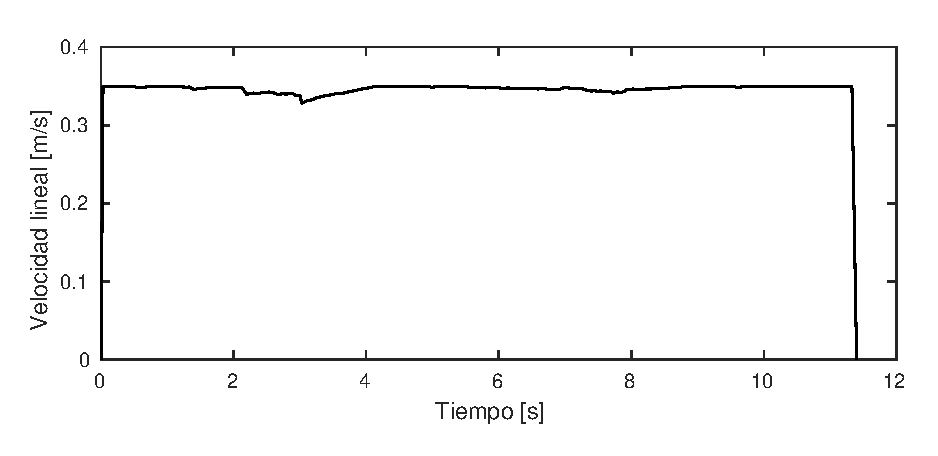
\includegraphics[width=0.45\textwidth]{Figures/SpeedWithoutProfile.eps}
    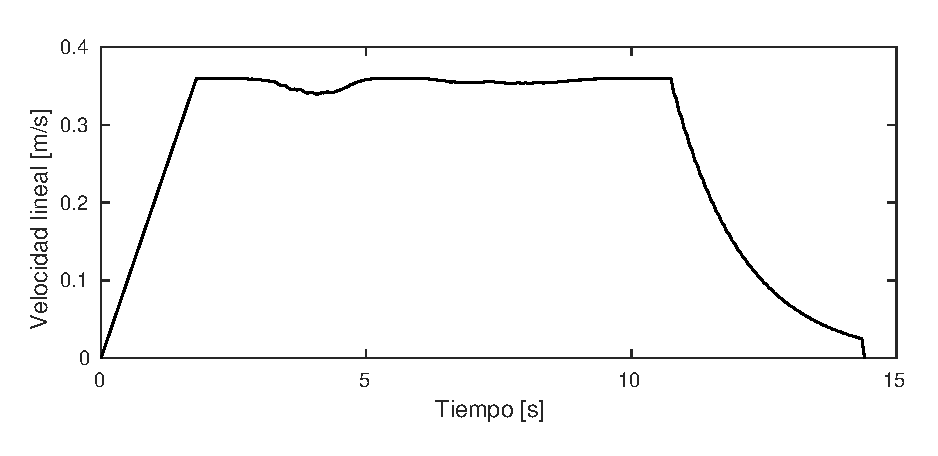
\includegraphics[width=0.45\textwidth]{Figures/SpeedWithProfile.eps}
  \end{figure}
\end{frame}

\section{Evasión de obstáculos}
\begin{frame}\frametitle{Evasión de obstáculos}
  \begin{itemize}
  \item Hasta el momento se tiene una manera de representar el ambiente, planear una ruta y seguirla
  \item ¿Qué pasa si en el ambiente hay un obstáculo que no estaba en el mapa?
  \item Se requiere de una técnica reactiva para evadir obstáculos
  \item Una posible solución es el uso de campos potenciales artificiales
  \end{itemize}
\end{frame}

\begin{frame}\frametitle{Campos potenciales artificiales}
  
\end{frame}

\bibliographystyle{abbrv}
\bibliography{References}
\begin{frame}
  \Huge{Gracias}
  \[\]
  \Large{Contacto}
  \[\]
  \large
  Dr. Marco Negrete\\
  Profesor Asociado C\\
  Departamento de Procesamiento de Señales\\
  Facultad de Ingeniería, UNAM.
\[\]
mnegretev.info\\
marco.negrete@ingenieria.unam.edu\\
\end{frame}
\end{document}
